\chapter{Introduzione a Git e Version Control}

\section*{Introduzione}
Il version control (controllo di versione) è una pratica fondamentale nello sviluppo software moderno. Git rappresenta lo standard de facto per tracciare modifiche al codice, collaborare con altri sviluppatori e gestire progetti di qualsiasi dimensione. Questo capitolo introduce i concetti fondamentali del version control, la storia di Git e le differenze tra sistemi centralizzati e distribuiti.

\section*{Obiettivi di apprendimento}
\begin{itemize}
    \item Comprendere cos'è il version control e perché è necessario
    \item Conoscere la storia e l'evoluzione di Git
    \item Distinguere tra VCS centralizzati e distribuiti
    \item Comprendere l'architettura di Git
    \item Conoscere i vantaggi di Git rispetto ad altri VCS
    \item Configurare Git per la prima volta
\end{itemize}

\section{Cos'è il Version Control}

\subsection{Definizione}
Un \textbf{Version Control System (VCS)} è un software che registra le modifiche ai file nel tempo, permettendo di richiamare versioni specifiche in un secondo momento. È come una macchina del tempo per il codice sorgente.

\subsection{Il problema senza version control}

Immagina di lavorare su un progetto senza version control:

\begin{lstlisting}[caption=Cartella progetto senza VCS]
mio-progetto/
  main.py
  main_v2.py
  main_v2_final.py
  main_v2_final_REALMENTE_FINALE.py
  main_v2_final_REALMENTE_FINALE_fix.py
  main_backup_20241110.py
\end{lstlisting}

\textbf{Problemi evidenti}:
\begin{itemize}
    \item Impossibile sapere cosa è cambiato tra versioni
    \item Nessuna traccia di chi ha fatto modifiche
    \item Difficile collaborare (chi ha la versione corretta?)
    \item Nessun modo di tornare indietro facilmente
    \item Naming chaos totale
\end{itemize}

\begin{tcolorbox}[colback=red!10, colframe=red!60, title=Errore Comune: Version Control Manuale]
Creare copie manuali dei file con suffissi come \texttt{\_v1}, \texttt{\_final}, \texttt{\_backup} è inefficiente, error-prone e non scala. Il version control automatizza questo processo in modo robusto e professionale.
\end{tcolorbox}

\subsection{La soluzione: Version Control System}

Con un VCS come Git:
\begin{itemize}
    \item \textbf{Tracking automatico}: Ogni modifica è tracciata con timestamp e autore
    \item \textbf{Commit messages}: Descrizioni di cosa è stato modificato e perché
    \item \textbf{Branching}: Lavorare su feature diverse in parallelo senza conflitti
    \item \textbf{Rollback}: Tornare a versioni precedenti istantaneamente
    \item \textbf{Collaborazione}: Più persone lavorano sugli stessi file senza sovrascriversi
    \item \textbf{Storia completa}: Audit trail di tutto il progetto
\end{itemize}

\begin{tcolorbox}[colback=blue!10, colframe=blue!60, title=Esempio Pratico]
Stai sviluppando una funzionalità ma scopri un bug critico in produzione. Con Git:
\begin{enumerate}
    \item Salvi il lavoro corrente (\texttt{git stash})
    \item Torni alla versione di produzione (\texttt{git checkout main})
    \item Crei un hotfix branch (\texttt{git checkout -b hotfix/critical-bug})
    \item Fixxi il bug e fai push
    \item Torni alla tua feature (\texttt{git checkout feature/nuova-funzione})
    \item Recuperi il lavoro salvato (\texttt{git stash pop})
\end{enumerate}

Tutto in pochi secondi, senza perdere nulla!
\end{tcolorbox}

\section{Storia di Git}

\subsection{Pre-Git: BitKeeper e la crisi del 2005}

Il kernel Linux (1991-2005) inizialmente usava patch e archivi tar per gestire contributi. Nel 2002, il progetto adottò BitKeeper, un VCS proprietario che offriva licenze gratuite ai sviluppatori open source.

\textbf{La crisi del 2005}: BitKeeper revocò le licenze gratuite dopo controversie con la community. Linus Torvalds si trovò senza VCS adeguato per gestire migliaia di contributi al kernel.

\subsection{Nascita di Git (Aprile 2005)}

Linus Torvalds decise di creare un nuovo VCS con questi obiettivi:
\begin{itemize}
    \item \textbf{Velocità}: Operazioni locali istantanee
    \item \textbf{Design semplice}: Architettura comprensibile
    \item \textbf{Supporto branching non lineare}: Migliaia di branch paralleli
    \item \textbf{Completamente distribuito}: Nessun server centrale obbligatorio
    \item \textbf{Gestione progetti grandi}: Kernel Linux ha 25+ milioni linee di codice
\end{itemize}

\textbf{Timeline}:
\begin{itemize}
    \item \textbf{3 Aprile 2005}: Linus inizia a scrivere Git
    \item \textbf{7 Aprile 2005}: Git diventa self-hosting (gestisce il proprio codice)
    \item \textbf{16 Giugno 2005}: Kernel Linux 2.6.12 rilasciato usando Git
    \item \textbf{21 Luglio 2005}: Linus passa la manutenzione a Junio Hamano
    \item \textbf{2008-oggi}: Git diventa lo standard de facto
\end{itemize}

\begin{tcolorbox}[colback=green!10, colframe=green!60, title=Fun Fact]
Linus Torvalds ha scritto la prima versione funzionante di Git in \textbf{10 giorni}. Il nome "git" è slang britannico per "persona testarda/antipatica" - Linus scherzosamente dice: "I name all my projects after myself: first Linux, now Git."
\end{tcolorbox}

\subsection{Evoluzione e adozione}

\begin{description}
    \item[2008] GitHub lanciato - hosting gratuito per repository Git
    \item[2011] GitLab lanciato - alternativa self-hosted
    \item[2018] Microsoft acquisisce GitHub per 7.5 miliardi di dollari
    \item[2020+] Git è usato da 90\%+ dei progetti software professionali
\end{description}

\section{VCS Centralizzati vs Distribuiti}

\subsection{Version Control System Centralizzati (CVCS)}

Esempi: \textbf{SVN (Subversion)}, CVS, Perforce

\textbf{Architettura}:
\begin{figure}[h]
    \centering
    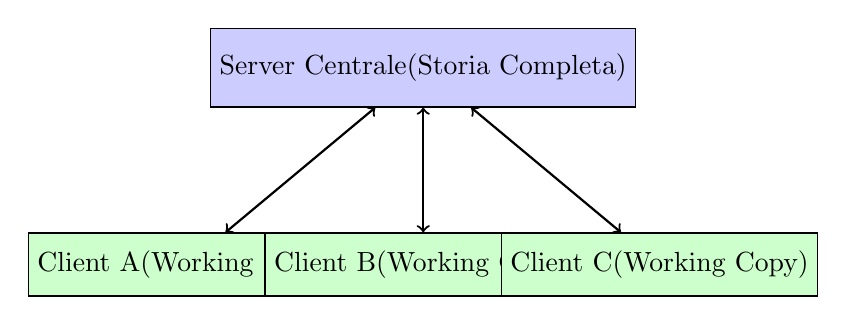
\begin{tikzpicture}[
        server/.style={rectangle, draw, fill=blue!20, minimum width=2.5cm, minimum height=1cm},
        client/.style={rectangle, draw, fill=green!20, minimum width=2cm, minimum height=0.8cm}
    ]
        % Server centrale
        \node[server] (server) at (0,0) {Server Centrale\\(Storia Completa)};

        % Client
        \node[client] (client1) at (-3,-2.5) {Client A\\(Working Copy)};
        \node[client] (client2) at (0,-2.5) {Client B\\(Working Copy)};
        \node[client] (client3) at (3,-2.5) {Client C\\(Working Copy)};

        % Connessioni
        \draw[<->, thick] (server) -- (client1);
        \draw[<->, thick] (server) -- (client2);
        \draw[<->, thick] (server) -- (client3);
    \end{tikzpicture}
    \caption{Architettura CVCS - Server Centrale}
\end{figure}

\textbf{Caratteristiche CVCS}:
\begin{itemize}
    \item Un server centrale contiene tutta la storia
    \item I client hanno solo l'ultima versione (working copy)
    \item Ogni operazione richiede connessione al server
    \item Commit = push immediato al server
\end{itemize}

\textbf{Vantaggi CVCS}:
\begin{itemize}
    \item Amministrazione centralizzata (controllo accessi)
    \item Modello mentale semplice
    \item Backup centralizzato
\end{itemize}

\textbf{Svantaggi CVCS}:
\begin{itemize}
    \item \textbf{Single Point of Failure}: Server down = nessuno lavora
    \item \textbf{Richiede rete}: Impossibile commit offline
    \item \textbf{Lento}: Ogni diff/log richiede query al server
    \item \textbf{Branching costoso}: Creare branch è pesante
    \item \textbf{Rischio perdita dati}: Se il server crasha, si perde tutto
\end{itemize}

\subsection{Version Control System Distribuiti (DVCS)}

Esempi: \textbf{Git}, Mercurial, Bazaar

\textbf{Architettura}:
\begin{figure}[h]
    \centering
    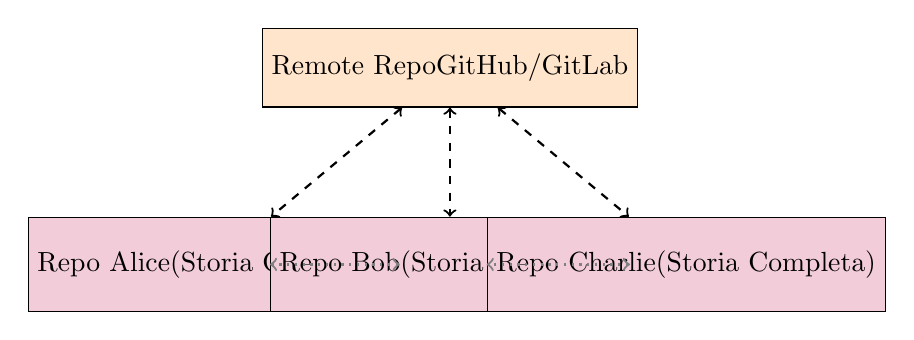
\begin{tikzpicture}[
        repo/.style={rectangle, draw, fill=purple!20, minimum width=2.2cm, minimum height=1.2cm},
        remote/.style={rectangle, draw, fill=orange!20, minimum width=2.5cm, minimum height=1cm}
    ]
        % Remote repository
        \node[remote] (remote) at (0,0) {Remote Repo\\GitHub/GitLab};

        % Local repositories
        \node[repo] (repo1) at (-3,-2.5) {Repo Alice\\(Storia Completa)};
        \node[repo] (repo2) at (0,-2.5) {Repo Bob\\(Storia Completa)};
        \node[repo] (repo3) at (3,-2.5) {Repo Charlie\\(Storia Completa)};

        % Connessioni
        \draw[<->, thick, dashed] (remote) -- (repo1);
        \draw[<->, thick, dashed] (remote) -- (repo2);
        \draw[<->, thick, dashed] (remote) -- (repo3);

        % Connessioni peer-to-peer (opzionali)
        \draw[<->, thick, dotted, gray] (repo1) -- (repo2);
        \draw[<->, thick, dotted, gray] (repo2) -- (repo3);
    \end{tikzpicture}
    \caption{Architettura DVCS - Distribuita}
\end{figure}

\textbf{Caratteristiche DVCS}:
\begin{itemize}
    \item Ogni clone è una copia completa del repository (storia inclusa)
    \item Operazioni locali (commit, branch, merge) istantanee
    \item Sincronizzazione esplicita (push/pull)
    \item Possibilità di lavorare offline
\end{itemize}

\textbf{Vantaggi DVCS}:
\begin{itemize}
    \item \textbf{Backup naturale}: Ogni clone è un backup completo
    \item \textbf{Velocità}: Operazioni locali senza latenza di rete
    \item \textbf{Offline-first}: Lavoro completo senza connessione
    \item \textbf{Branching leggero}: Creare branch è istantaneo
    \item \textbf{Flessibilità workflow}: Supporta workflow complessi
    \item \textbf{Integrità}: Checksum garantisce nessuna corruzione
\end{itemize}

\textbf{Svantaggi DVCS}:
\begin{itemize}
    \item Curva di apprendimento più ripida
    \item Concetti più complessi (staging area, rebase, etc.)
    \item Storage locale maggiore (tutta la storia)
\end{itemize}

\begin{tcolorbox}[colback=purple!10, colframe=purple!60, title=Confronto CVCS vs DVCS]
\begin{tabular}{lll}
\textbf{Caratteristica} & \textbf{CVCS (SVN)} & \textbf{DVCS (Git)} \\
\hline
Velocità operazioni & Lenta (rete) & Veloce (locale) \\
Lavoro offline & Limitato & Completo \\
Branching & Pesante & Leggero \\
Backup & Centralizzato & Distribuito \\
Curva apprendimento & Bassa & Media-Alta \\
Integrità dati & Buona & Eccellente \\
\end{tabular}
\end{tcolorbox}

\section{Architettura e Concetti Fondamentali di Git}

\subsection{I tre stati di Git}

Git ha tre stati principali in cui i file possono trovarsi:

\begin{figure}[h]
    \centering
    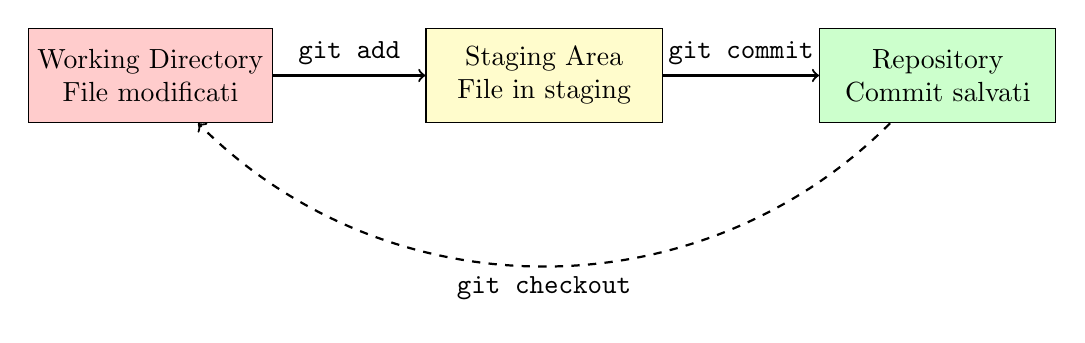
\begin{tikzpicture}[
        state/.style={rectangle, draw, minimum width=3cm, minimum height=1.2cm, align=center},
        arrow/.style={->, thick}
    ]
        \node[state, fill=red!20] (working) at (0,0) {Working Directory\\File modificati};
        \node[state, fill=yellow!20] (staging) at (5,0) {Staging Area\\File in staging};
        \node[state, fill=green!20] (repo) at (10,0) {Repository\\Commit salvati};

        \draw[arrow] (working) -- node[above] {\texttt{git add}} (staging);
        \draw[arrow] (staging) -- node[above] {\texttt{git commit}} (repo);
        \draw[arrow, dashed] (repo) to[bend left=45] node[below] {\texttt{git checkout}} (working);
    \end{tikzpicture}
    \caption{I tre stati di Git}
\end{figure}

\begin{description}
    \item[\textbf{Working Directory}] La directory di lavoro dove modifichi i file
    \item[\textbf{Staging Area (Index)}] Area intermedia dove prepari i file per il commit
    \item[\textbf{Repository (.git directory)}] Database dove Git salva snapshot (commit)
\end{description}

\subsection{Workflow base di Git}

\begin{enumerate}
    \item \textbf{Modifichi} file nella working directory
    \item \textbf{Staging}: Aggiungi snapshot dei file alla staging area (\texttt{git add})
    \item \textbf{Commit}: Salvi permanentemente snapshot nel repository (\texttt{git commit})
\end{enumerate}

\begin{lstlisting}[caption=Workflow tipico Git]
# Modifica file
$ echo "Hello Git" > README.md

# Visualizza stato
$ git status
# Output: README.md modificato (modified)

# Aggiungi alla staging area
$ git add README.md

# Visualizza stato
$ git status
# Output: README.md pronto per commit (staged)

# Commit con messaggio
$ git commit -m "Add greeting to README"

# Visualizza stato
$ git status
# Output: Working directory clean
\end{lstlisting}

\subsection{Snapshot, non differenze}

\textbf{Differenza fondamentale}: La maggior parte dei VCS (SVN, CVS) memorizza informazioni come lista di modifiche ai file (delta-based).

\textbf{Git} invece pensa ai dati come \textbf{snapshot} del filesystem. Ogni commit è una foto completa di tutti i file in quel momento.

\begin{figure}[h]
    \centering
    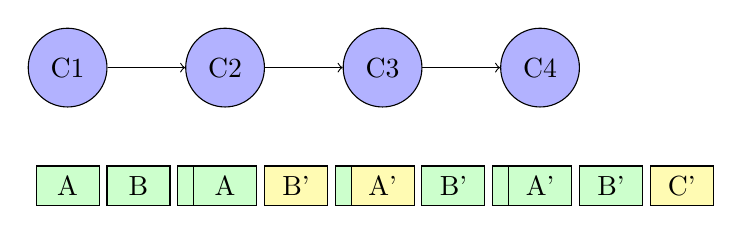
\begin{tikzpicture}[
        commit/.style={circle, draw, fill=blue!30, minimum size=1cm},
        file/.style={rectangle, draw, fill=gray!20, minimum width=0.8cm, minimum height=0.5cm}
    ]
        % Commits
        \node[commit] (c1) at (0,0) {C1};
        \node[commit] (c2) at (2,0) {C2};
        \node[commit] (c3) at (4,0) {C3};
        \node[commit] (c4) at (6,0) {C4};

        % Files in each commit
        \node[file, fill=green!20] at (0,-1.5) {A};
        \node[file, fill=green!20] at (0.9,-1.5) {B};
        \node[file, fill=green!20] at (1.8,-1.5) {C};

        \node[file, fill=green!20] at (2,-1.5) {A};
        \node[file, fill=yellow!30] at (2.9,-1.5) {B'};
        \node[file, fill=green!20] at (3.8,-1.5) {C};

        \node[file, fill=yellow!30] at (4,-1.5) {A'};
        \node[file, fill=green!20] at (4.9,-1.5) {B'};
        \node[file, fill=green!20] at (5.8,-1.5) {C};

        \node[file, fill=green!20] at (6,-1.5) {A'};
        \node[file, fill=green!20] at (6.9,-1.5) {B'};
        \node[file, fill=yellow!30] at (7.8,-1.5) {C'};

        \draw[->] (c1) -- (c2);
        \draw[->] (c2) -- (c3);
        \draw[->] (c3) -- (c4);
    \end{tikzpicture}
    \caption{Git: Snapshot completi ad ogni commit (giallo = modificato)}
\end{figure}

\textbf{Vantaggi snapshot}:
\begin{itemize}
    \item Checkout velocissimo (copia file, non ricostruisce da delta)
    \item Branching istantaneo (solo puntatori)
    \item Integrità garantita (checksum SHA-1 su tutto)
\end{itemize}

\subsection{Integrità e checksum SHA-1}

Ogni oggetto in Git è identificato da un \textbf{hash SHA-1} (160 bit, 40 caratteri esadecimali).

\begin{lstlisting}[caption=Esempio commit hash]
$ git log --oneline
a3f5b21 Add user authentication feature
b8c9d34 Fix navbar responsive layout
c7e2a19 Initial commit
\end{lstlisting}

\textbf{Proprietà SHA-1}:
\begin{itemize}
    \item Univoco: Probabilità collisione $\approx$ 0
    \item Immutabile: Modificare un byte cambia completamente l'hash
    \item Verificabile: Corruzione dati è immediatamente rilevata
\end{itemize}

\begin{tcolorbox}[colback=green!10, colframe=green!60, title=Best Practice: Integrità]
Git garantisce che non puoi modificare contenuti senza che Git lo sappia. È praticamente impossibile corrompere dati o avere modifiche non tracciate. Questo rende Git estremamente affidabile per progetti critici.
\end{tcolorbox}

\section{Perché Git è lo standard}

\subsection{Confronto con alternative}

\begin{description}
    \item[\textbf{Git vs SVN}] Git è più veloce, supporta branching leggero, lavoro offline completo
    \item[\textbf{Git vs Mercurial}] Sintassi simile, Git ha ecosistema più grande (GitHub)
    \item[\textbf{Git vs Perforce}] Git è gratuito e open source, Perforce migliore per asset binari enormi
\end{description}

\subsection{Adozione nel mondo reale}

\textbf{Statistiche}:
\begin{itemize}
    \item \textbf{90\%+} dei progetti software usano Git
    \item \textbf{100 milioni+} repository su GitHub (2023)
    \item Progetti famosi: Linux Kernel, Android, Windows, VS Code, React, TensorFlow
\end{itemize}

\section{Configurazione Iniziale di Git}

\subsection{Configurazione utente (obbligatoria)}

Ogni commit in Git contiene informazioni sull'autore. Configurazione richiesta:

\begin{lstlisting}[caption=Configurazione base Git]
# Configura nome (apparirà nei commit)
$ git config --global user.name "Mario Rossi"

# Configura email (apparirà nei commit)
$ git config --global user.email "mario.rossi@example.com"

# Verifica configurazione
$ git config --list
user.name=Mario Rossi
user.email=mario.rossi@example.com
\end{lstlisting}

\subsection{Livelli di configurazione}

Git ha tre livelli di configurazione:

\begin{description}
    \item[\texttt{--system}] Configurazione globale per tutti gli utenti del sistema\\
    File: \texttt{/etc/gitconfig}

    \item[\texttt{--global}] Configurazione per l'utente corrente\\
    File: \texttt{\~{}/.gitconfig} o \texttt{\~{}/.config/git/config}

    \item[\texttt{--local}] Configurazione per il repository specifico (default)\\
    File: \texttt{.git/config} nel repository
\end{description}

Le configurazioni local sovrascrivono global, che sovrascrive system.

\subsection{Configurazioni utili}

\begin{lstlisting}[caption=Altre configurazioni consigliate]
# Editor di default per commit message (esempio: vim, nano, code)
$ git config --global core.editor "code --wait"

# Colori output Git
$ git config --global color.ui auto

# Default branch name (main invece di master)
$ git config --global init.defaultBranch main

# Autocorrect comandi (attende 1.5 secondi prima di eseguire)
$ git config --global help.autocorrect 15

# Alias utili
$ git config --global alias.st status
$ git config --global alias.co checkout
$ git config --global alias.br branch
$ git config --global alias.cm commit
$ git config --global alias.lg "log --oneline --graph --all"

# Dopo configurazione alias:
$ git st  # Equivalente a: git status
$ git lg  # Log grafico compatto
\end{lstlisting}

\subsection{Visualizzare e modificare configurazione}

\begin{lstlisting}[caption=Gestione configurazione]
# Visualizza tutte le configurazioni
$ git config --list

# Visualizza configurazione specifica
$ git config user.name
Mario Rossi

# Visualizza origine configurazione
$ git config --list --show-origin
file:/home/mario/.gitconfig user.name=Mario Rossi
file:/home/mario/.gitconfig user.email=mario.rossi@example.com

# Rimuovi configurazione
$ git config --global --unset user.email

# Modifica direttamente file configurazione
$ git config --global --edit
\end{lstlisting}

\section*{Riepilogo concetti chiave}

\begin{tcolorbox}[colback=gray!10, colframe=black!60, title=Concetti fondamentali]
\begin{itemize}
    \item \textbf{Version Control} traccia modifiche ai file nel tempo
    \item \textbf{Git} è un DVCS (Distributed Version Control System)
    \item Ogni clone Git contiene la \textbf{storia completa} del progetto
    \item Git usa \textbf{snapshot}, non differenze tra file
    \item I tre stati: \textbf{Working Directory}, \textbf{Staging Area}, \textbf{Repository}
    \item \textbf{SHA-1 checksum} garantisce integrità dei dati
    \item DVCS è superiore a CVCS per velocità, offline work, branching
    \item Configurare \texttt{user.name} e \texttt{user.email} è \textbf{obbligatorio}
\end{itemize}
\end{tcolorbox}

\section*{Esercizi}

\begin{enumerate}
    \item Spiega con un esempio pratico perché il version control è necessario in un progetto software.

    \item Descrivi le differenze tra VCS centralizzati (SVN) e distribuiti (Git). Quali sono i vantaggi di Git?

    \item Disegna un diagramma che mostra i tre stati di Git (Working Directory, Staging Area, Repository) e i comandi per passare da uno all'altro.

    \item Installa Git sul tuo computer e verifica la versione installata con \texttt{git --version}.

    \item Configura Git con il tuo nome ed email usando \texttt{git config --global}.

    \item Crea almeno 3 alias Git utili (esempio: \texttt{st} per status, \texttt{lg} per log grafico).

    \item Ricerca la storia di Git: perché Linus Torvalds ha creato Git nel 2005? Quali erano i requisiti che doveva soddisfare?

    \item Confronta Git con un altro VCS (Mercurial o SVN). Quali sono le differenze architetturali?

    \item Spiega cosa significa che Git usa "snapshot" invece di "differenze". Qual è il vantaggio?

    \item Visualizza tutte le tue configurazioni Git con \texttt{git config --list --show-origin} e identifica dove sono salvate.
\end{enumerate}

\section*{Verifica}

\textbf{Domande Vero/Falso}:
\begin{enumerate}
    \item Git è un sistema di version control centralizzato. (V/F)
    \item Ogni clone Git contiene la storia completa del repository. (V/F)
    \item La staging area è opzionale in Git. (V/F)
    \item SHA-1 garantisce l'integrità dei dati in Git. (V/F)
    \item Git richiede connessione internet per fare commit. (V/F)
    \item Linus Torvalds ha creato Git nel 2005. (V/F)
\end{enumerate}

\textbf{Domande a Risposta Multipla}:
\begin{enumerate}
    \item Quale comando configura il nome utente globalmente?
    \begin{itemize}
        \item \texttt{git config user.name "Nome"}
        \item \texttt{git config --global user.name "Nome"}
        \item \texttt{git set --global user.name "Nome"}
        \item \texttt{git user.name "Nome"}
    \end{itemize}

    \item Cosa memorizza Git ad ogni commit?
    \begin{itemize}
        \item Solo le differenze tra file
        \item Snapshot completo di tutti i file
        \item Solo i nomi dei file modificati
        \item Compressione dei file
    \end{itemize}
\end{enumerate}

\section*{Laboratorio pratico}

\textbf{Lab 1: Setup ambiente Git}

\begin{enumerate}
    \item Installa Git sul tuo sistema operativo
    \item Verifica l'installazione: \texttt{git --version}
    \item Configura nome ed email globalmente
    \item Configura editor di default (es: VS Code, Vim, Nano)
    \item Crea 5 alias personalizzati
    \item Visualizza tutte le configurazioni e salva l'output in un file
    \item Sperimenta con \texttt{git config --global --edit}
\end{enumerate}

\section*{Riferimenti}

\begin{itemize}
    \item Pro Git Book: \url{https://git-scm.com/book/it/v2}
    \item Git Official Documentation: \url{https://git-scm.com/doc}
    \item Git History (Linus Torvalds): \url{https://git-scm.com/book/en/v2/Getting-Started-A-Short-History-of-Git}
    \item Visualizing Git: \url{https://git-school.github.io/visualizing-git/}
    \item GitHub Learning Lab: \url{https://lab.github.com}
\end{itemize}
